\documentclass[13spt]{beamer}

%packages
\usepackage[utf8]{inputenc}
\usepackage{amsmath}
\usepackage{amsfonts}
\usepackage{amssymb}
\usepackage{graphicx}
\usepackage{caption}
\usepackage{booktabs}
\usepackage[vietnamese]{babel}

%use
\usetheme{Warsaw}
\definecolor{ballblue}{rgb}{0.13, 0.67, 0.8}
\definecolor{azure(colorwheel)}{rgb}{0.0, 0.5, 1.0}
\definecolor{blue(ryb)}{rgb}{0.01, 0.28, 1.0}
\definecolor{phthaloblue}{rgb}{0.0, 0.06, 0.54}
\usecolortheme[named =phthaloblue]{structure}

%---------------------------------------------------------------------------------------------------------------------------------------------------------
%begin
\begin{document}
\title{Bảo Vệ Khóa Luận Tốt Nghiệp} 
\subtitle {Tìm Hiểu Và Vận Dụng Phương Pháp Xử Lý Dữ Liệu Lớn }


\author[ Trịnh Đình Phúc]{  \hspace{7mm} GVHD \hspace{5mm}: Th.S Cao Mạnh Hùng\\[3mm]{\hspace{1mm}Sinh Viên : Trịnh Đình Phúc\\ \hspace{18mm} }}

\date{\today} 

\frame{\titlepage} 
%page number
\setbeamertemplate{sidebar right}{}
\setbeamertemplate{footline}{%
\hfill\usebeamertemplate***{navigation symbols}
\hspace{1cm}\insertframenumber{}/\inserttotalframenumber}

\frame{\frametitle{Mục Lục}\tableofcontents} 


\section{Giới thiệu đề tài} 
\subsection{Thế nào gọi là "Dữ liệu lớn"?}
\begin{frame}{Thế nào gọi là "Dữ liệu lớn"?}
\textbf{Thống kê:}
	\begin{itemize}
		\item 25+ TB được tạo ra mỗi giây trên toàn cầu.  
		\item 90+ \% dữ liệu của thế giới được tạo ra trong 2 năm vừa qua.
		\item 90+ \% dữ liệu được tạo ra là dữ liệu phi cấu trúc.
	\end{itemize}
\vspace{2mm}
\textbf{Các dạng dữ liệu:}
  \begin{tabular} {l l }
  \toprule
  \it Data & \it Ứng dụng trong việc khai thác \\
  \midrule
  Văn bản & Xử lý ngôn ngữ tự nhiên  \\
  Ảnh và Video & Thị giác máy tính  \\  
  Âm thanh & Xử lý tín hiệu số  \\
  Social Network & Phân tích đồ thị  \\  
  Business & Khai thác dữ liệu  \\
  DNA & Tin sinh học \\           
  ... & ...\\            
  \bottomrule
  \end{tabular}
	
\end{frame}
\subsection{Làm thế nào để khai thác "Dữ liệu lớn"?}
%\begin{frame}{Làm thế nào để khai thác "Dữ liệu lớn"?}
%	\begin{figure}[h!]
%	  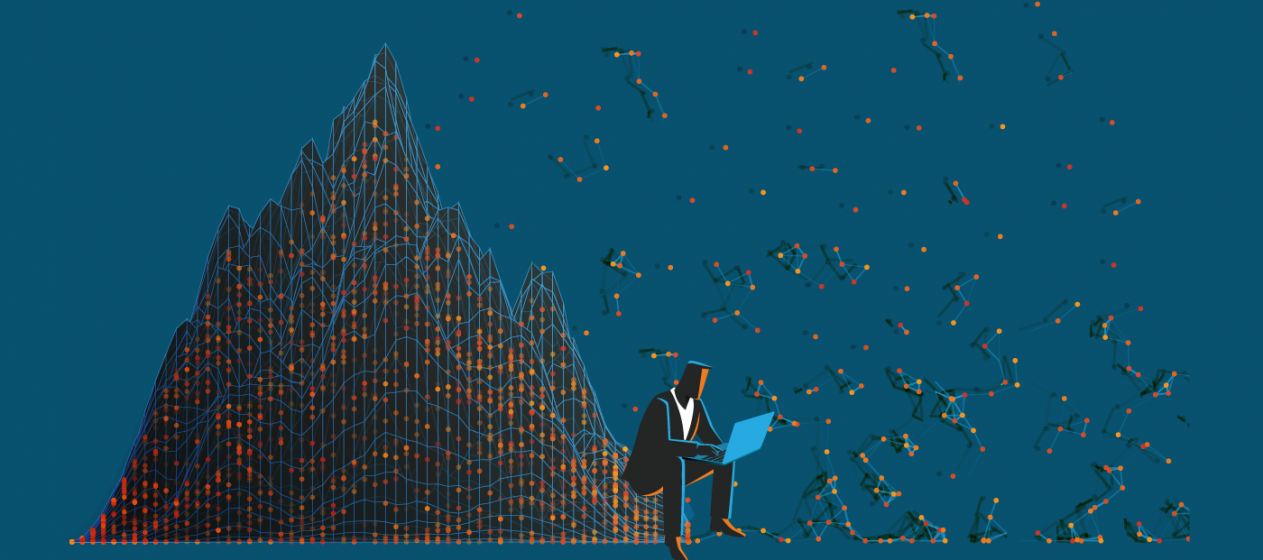
\includegraphics[width=0.9\linewidth]{bigdata.png}
%	  \caption{Làm sao để khai thác "Dữ liệu lớn"?}
%	  \label{fig:writing-thesis}
%	\end{figure}
%\end{frame}
\begin{frame}{Làm thế nào để khai thác "Dữ liệu lớn"?}
	\begin{figure}[h!]
	  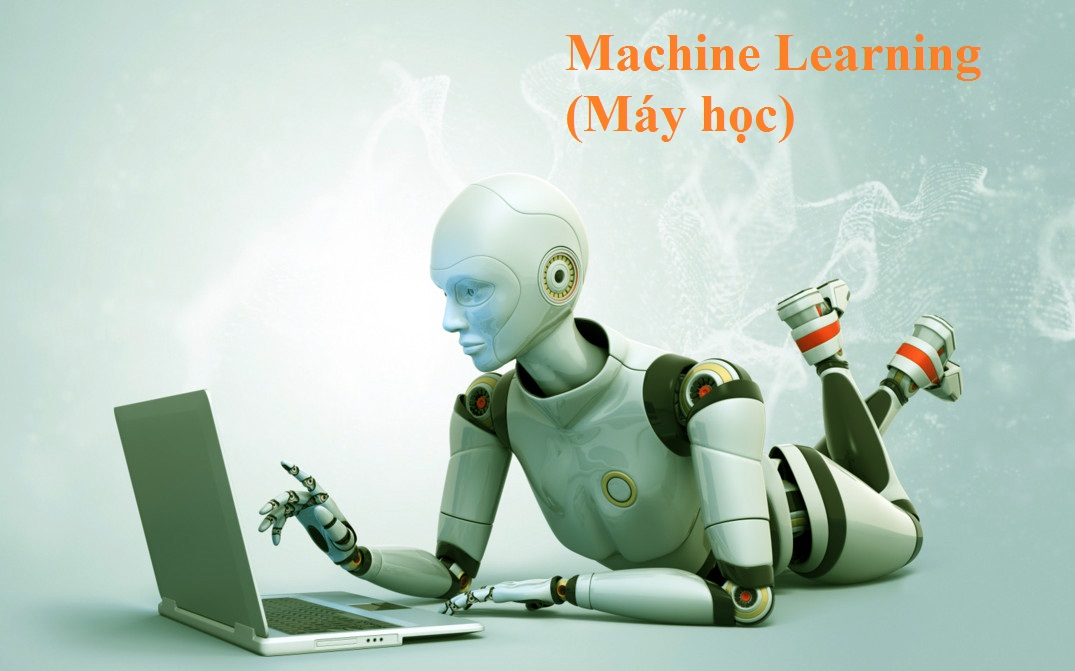
\includegraphics[width=0.9\linewidth]{machine-learning.jpg}
	  \caption{Máy học}
	  \label{fig:writing-thesis}
	\end{figure}
\end{frame}

\section{Các bước khai thác dữ liệu}
\frame{Các bước khai thác dữ liệu

 \begin{columns}
 \begin{column}{0.4\textwidth}
	\begin{figure}[h!]
	  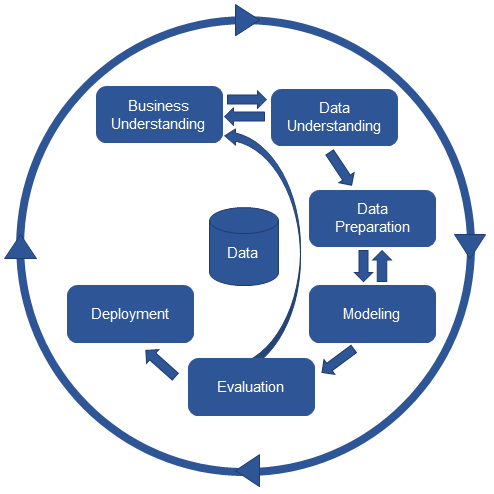
\includegraphics[width=0.9\linewidth,height=0.5\textheight,keepaspectratio]{CRISP-DM1.png}
	  \caption{Quy trình khai thác dữ liệu CRISP-DM (Cross Industry Standard Process for Data Mining)}
	  \label{fig:writing-thesis}
	\end{figure}
 \end{column}
  \begin{column}{0.6\textwidth}
  \begin{small}

	\textbf{Quy trình khai thác dữ liệu có 6 bước chính: \small}
	\begin{enumerate}
	\item Tìm hiểu nghiệp vụ (Business understanding) \pause 
	\item Tìm hiểu dữ liệu (Data understanding) \pause 
	\item Chuẩn bị dữ liệu (Data preparation) \pause 
	\item Mô hình hoá (Modeling)
		\begin{itemize}
		\item Input: Dữ liệu
		\item Output: Dự đoán tương lai, phân loại khách hàng, phát hiện hành vi giả mạo,... \pause
		\end{itemize}
	\item Đánh giá mô hình (Evaluation Model)\pause 
	\item Triển khai (Deployment)\pause 
	\end{enumerate}	
	\end{small}

 \end{column}
 \end{columns}

} 
\subsection{Thu thập dữ liệu}
\frame{\frametitle{Thu thập dữ liệu từ FIFA}
	\begin{figure}[h!]
	  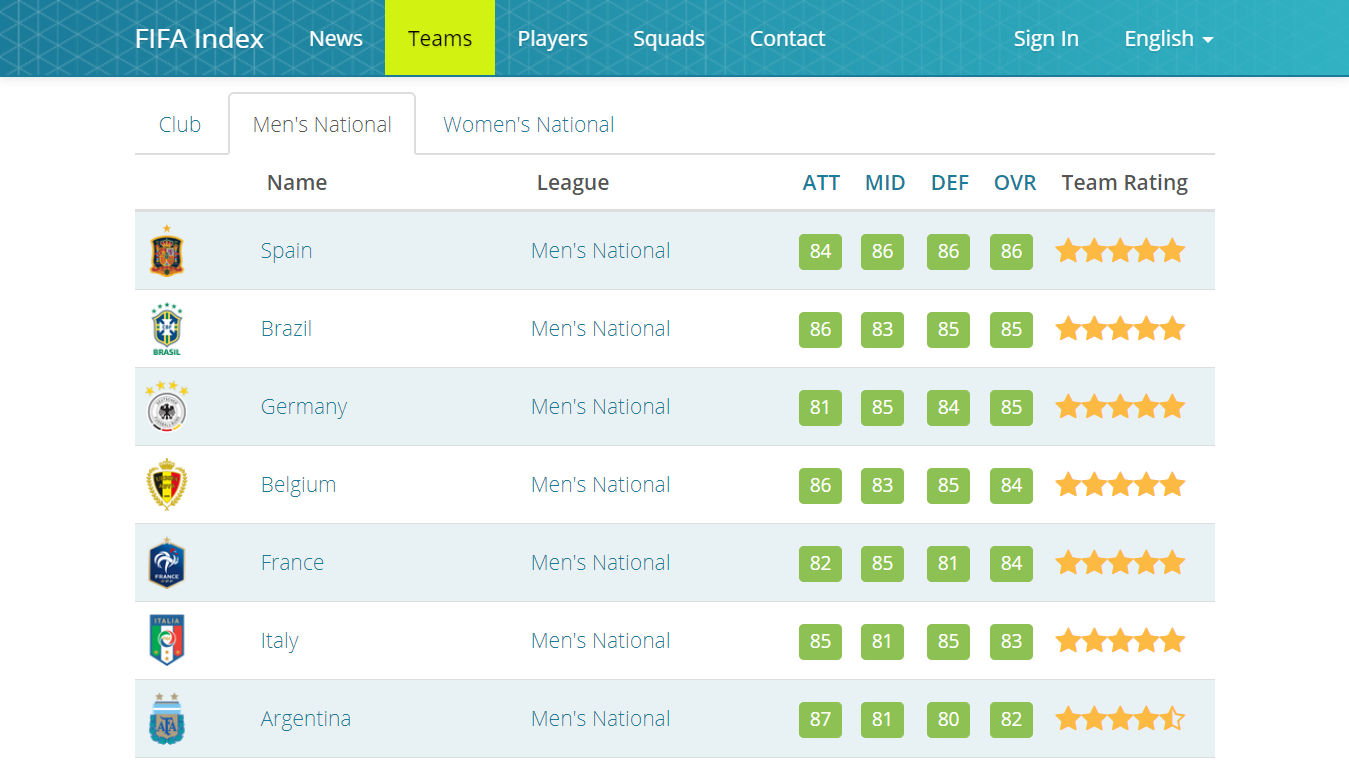
\includegraphics[width=1\linewidth,height=0.8\textheight,keepaspectratio]{fifa.png}
	  \caption{Dữ liệu từ liên đoàn bóng đá thế giới FIFA}
	  \label{fig:writing-thesis}
	\end{figure}
}

\frame{\frametitle{Thu thập dữ liệu từ Mendeley}
	\begin{figure}[h!]
	  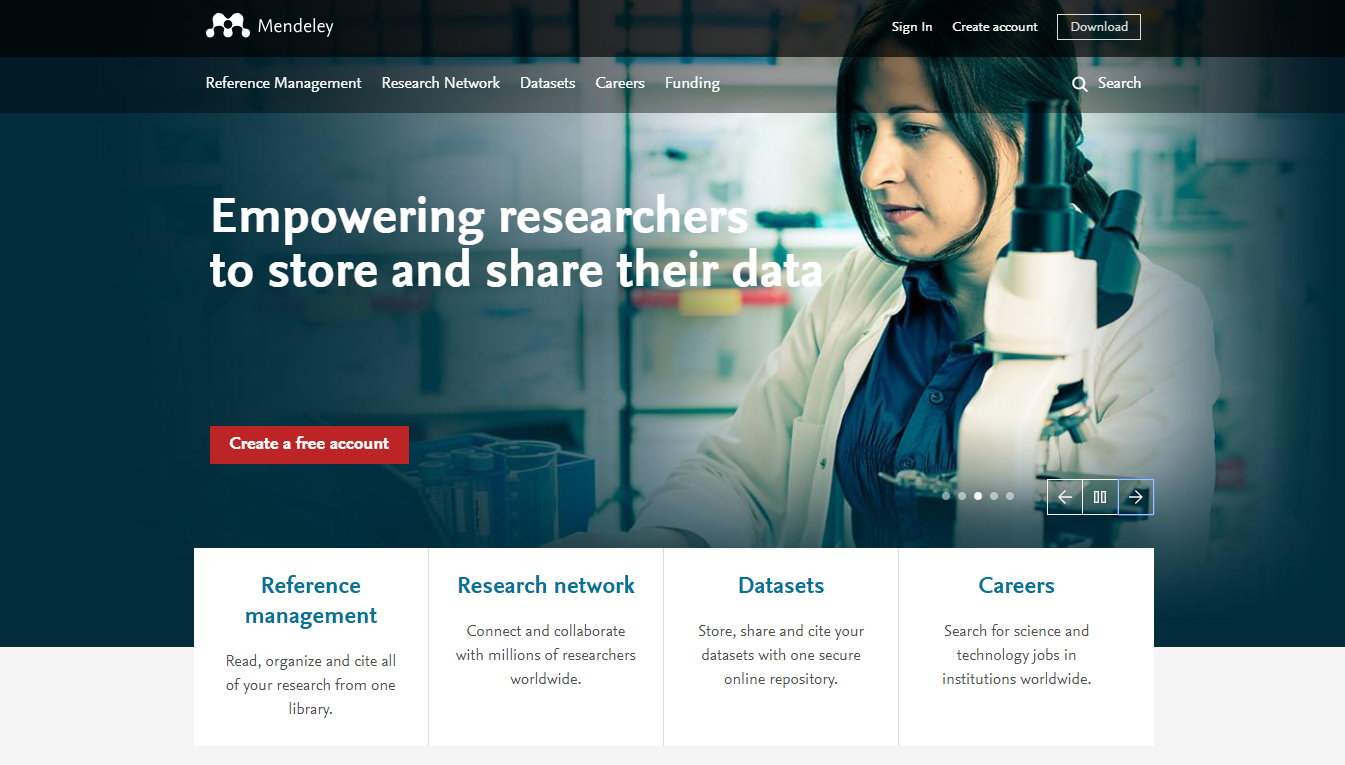
\includegraphics[width=1\linewidth,height=0.8\textheight,keepaspectratio]{X-Ray.png}
	   \caption{Dữ liệu từ mạng xã hội học thuật tổ chức nghiên cứu, cộng tác Mendeley}
	  \label{fig:writing-thesis}
	\end{figure}
}

\subsection{Tìm hiểu dữ liệu (Data understanding)}
\frame{\frametitle{Tìm hiểu dữ liệu (Data understanding)}
	\begin{figure}[h!]
	  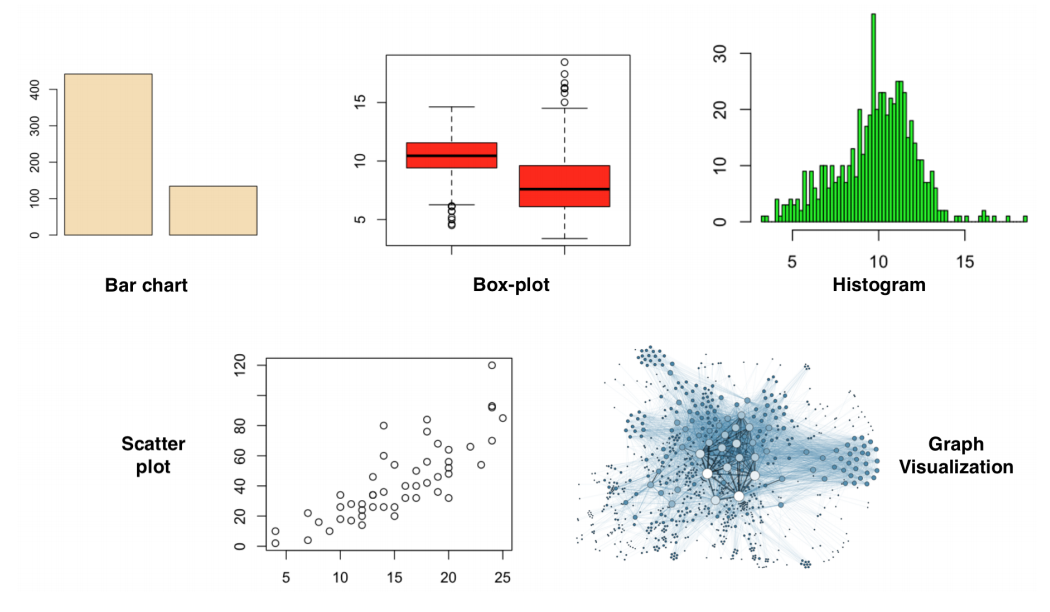
\includegraphics[width=1\linewidth,height=0.8\textheight,keepaspectratio]{plot.png}
	  \caption{Sử dụng các biểu đồ để phân tích}
	  \label{fig:writing-thesis}
	\end{figure}
}
\subsection{Chuẩn bị dữ liệu (Data preparation)}
\frame{\frametitle{Chuẩn bị dữ liệu (Data preparation)}
\begin{itemize}
\item Bag of word
\item TF-IDF
\item One-Hot-Encoding
\item Feature Scaling
\item Normalization
\item PCA
\item Feature Selection
\item Label Encoder
\end{itemize} 
}

\subsection{Mô hình hoá (Modeling)}
\frame{\frametitle{Machine Learning - Học}
	\begin{figure}[h!]
	  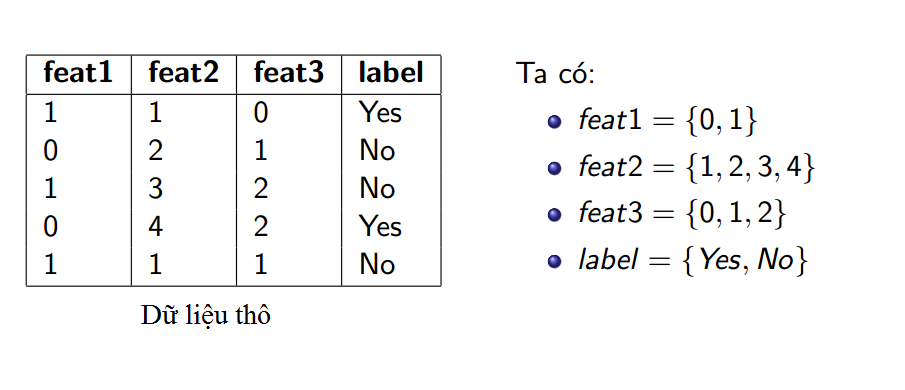
\includegraphics[width=1\linewidth,height=0.8\textheight,keepaspectratio]{modeling1.png}
	  \label{fig:writing-thesis}
	\end{figure}
}
\frame{\frametitle{Machine Learning - Dự đoán}
	\begin{figure}[h!]
	  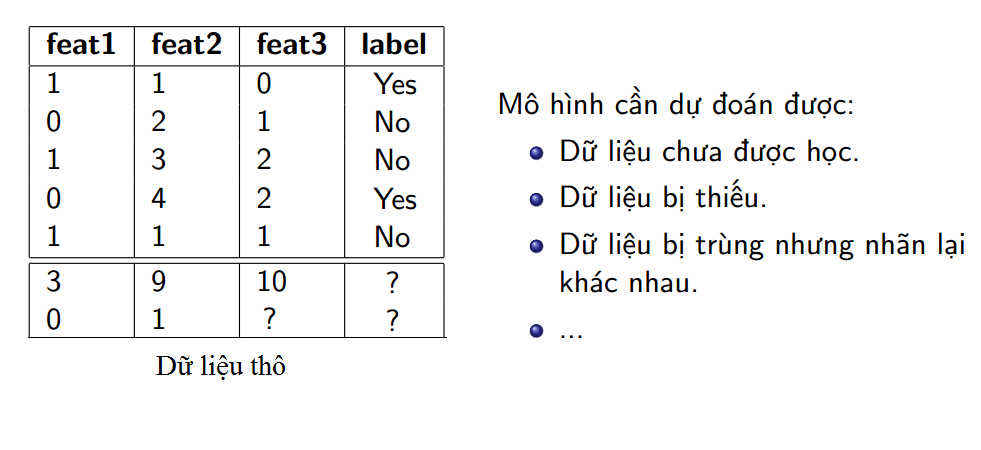
\includegraphics[width=1\linewidth,height=0.8\textheight,keepaspectratio]{modeling2.png}
	  \label{fig:writing-thesis}
	\end{figure}
}
\frame{\frametitle{Machine Learning - Thuật toán}
	\begin{figure}[h!]
	  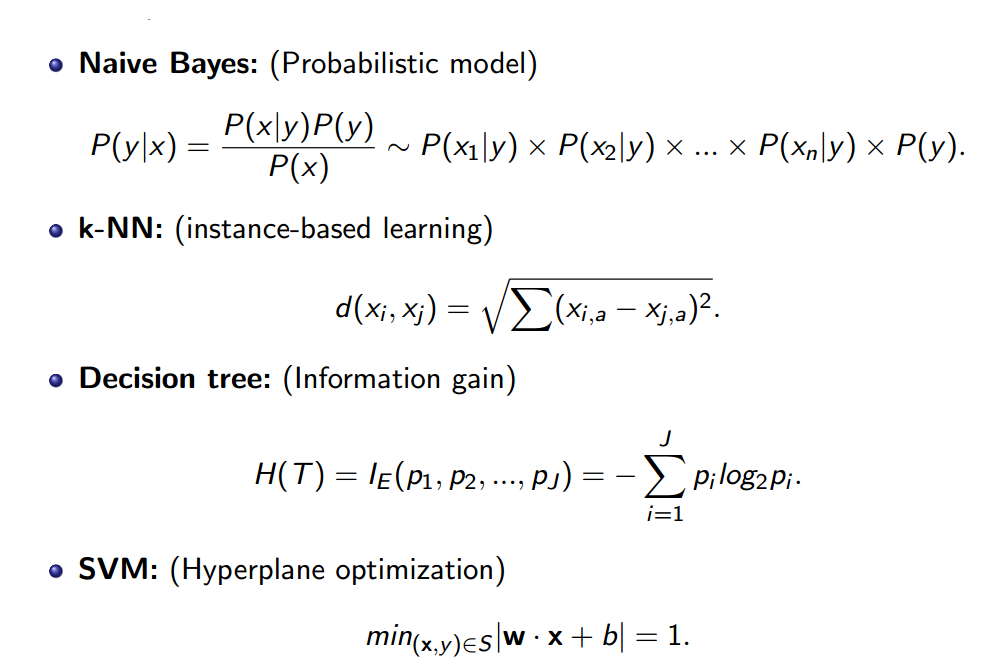
\includegraphics[width=1\linewidth,height=0.8\textheight,keepaspectratio]{modeling3.png}
	  \label{fig:writing-thesis}
	\end{figure}
}
\subsection{Đánh giá mô hình (Evaluation Model)}
\frame{\frametitle{Đánh giá mô hình)}
\begin{itemize}
\item Accuracy
\item Confusion Matrix (CM)
\item True/False Positive/Negative
\item Receiver operating characteristic curve (ROC)
\item Area Under the Curve
\item Precision và Recall
\item Residual sum of squares (RSS)
\end{itemize} 
}

\section{Kết quả đề tài} 
\frame{\frametitle{Kết quả đề tài}
 
}

\end{document}
%---------------------------------------------------------------------------------------------------------------------------------------------------------

